\documentclass{article}
\usepackage{tikz}
\usepackage{amsmath}

\begin{document}

\begin{center}
    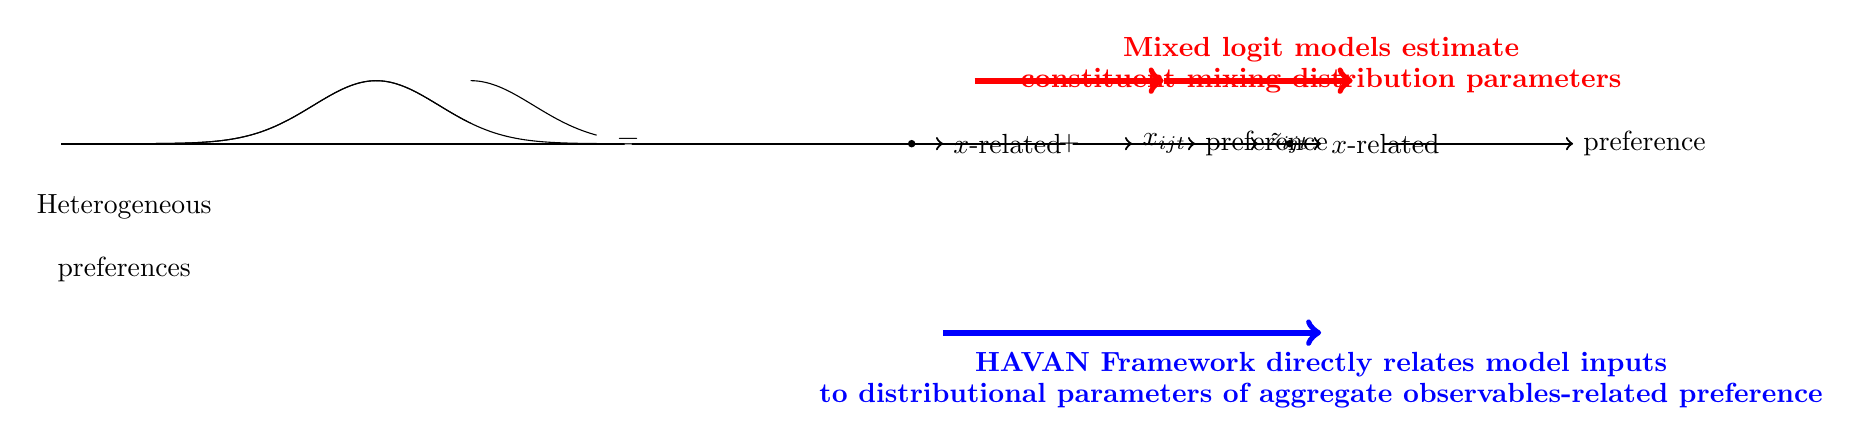
\begin{tikzpicture}[scale=0.8]
        % Preferences
        \draw[thick,->] (-5,0) -- (12,0) node[right] {$x_{ijt}$};
        \draw[thick,->] (7,0) -- (14,0) node[right] {$z_{ijt}$};
        \draw plot[domain=-3.5:3.5,samples=100] (\x,{exp(-(\x)^2/2)});
        \node at (-4,-1) {Heterogeneous};
        \node at (-4,-2) {preferences};
        
        % Equal sign
        \filldraw[white] (4,0) circle (0.05);
        \node at (4,0) {$=$};
        
        % Preference 1
        \draw[thick,->] (6,0) -- (9,0) node[right] {$x$-related};
        \draw[thick,->] (10,0) -- (13,0) node[right] {preference};
        \draw plot[domain=1.5:3.5,samples=100] (\x,{exp(-(\x-1.5)^2/2)});
        \filldraw (8.5,0) circle (0.05);
        
        % Plus sign
        \filldraw[white] (11,0) circle (0.05);
        \node at (11,0) {$+$};
        
        % Preference 2
        \draw[thick,->] (12,0) -- (15,0) node[right] {$x$-related};
        \draw[thick,->] (16,0) -- (19,0) node[right] {preference};
        \draw plot[domain=-3.5:1.5,samples=100] (\x,{exp(-(\x)^2/2)});
        \filldraw (14.5,0) circle (0.05);
        
        % Arrows
        \draw[red,->,line width=0.8mm] (9.5,1) -- (12.5,1);
        \draw[red,->,line width=0.8mm] (12.5,1) -- (15.5,1);
        
        % Text
        \node[red] at (15,1.5) {\textbf{Mixed logit models estimate}};
        \node[red] at (15,1) {\textbf{constituent mixing distribution parameters}};
        
        % HAVAN Framework
        \draw[blue,->,line width=0.8mm] (9,-3) -- (15,-3);
        \node[blue] at (15,-3.5) {\textbf{HAVAN Framework directly relates model inputs}};
        \node[blue] at (15,-4) {\textbf{to distributional parameters of aggregate observables-related preference}};
    \end{tikzpicture}
\end{center}

\end{document}